\chapter{Интеллектуальные системы регистрации и анализа проблемных ситуаций, возникающих в ИТ-инфраструктуре предприятия} \label{chapt1}

\section{Сравнительный анализ систем регистрации и устранения проблемных ситуаций} 
В данной главе рассматриваются имеющиеся на данный момент интеллектуальные системы регистрации и анализа проблемных ситуаций. \par
\textbf{HP OpenView} \cite{HPOpenView, HP1, HP2, HP3} является комплексным программным решением по мониторингу ИТ-инфраструктуры предприятия и имеет множество модулей. На рисунке \ref{img:hpopenview} представлен вид системы, которая обладает широким спектром возможностей: мониторинг \cite{HP4, HP5}; регистрация инцидентов; управление системами. Система не поддерживает: понимание и формализацию запросов; автоматическое устранение проблемы на основе формализации запроса.

\begin{figure} [h] 
  \center
  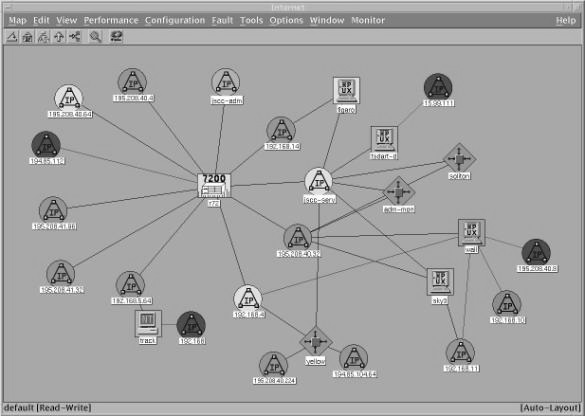
\includegraphics [scale=1.0] {hpopenview}
  \caption{HP OpenView} 
  \label{img:hpopenview}  
\end{figure}

Система \textbf{ServiceNOW}\footnote{Система ServiceNOW \url{http://www.servicenow.com/}}~--- средство автоматизации сервиса. На рисунке \ref{img:svnow} представлен вид этой системы, которая предоставляет следующие возможности: регистрация инцидентов и создание цепи их обработки. Система не поддерживает: понимание и формализацию запросов; автоматическое исправление проблемы на основе формализации запроса. Система широко используется в ИТ-инфраструктуре CERN \cite{SN1, SN2} для регистрации инцидентов и их решения.

\begin{figure} [h] 
  \center
  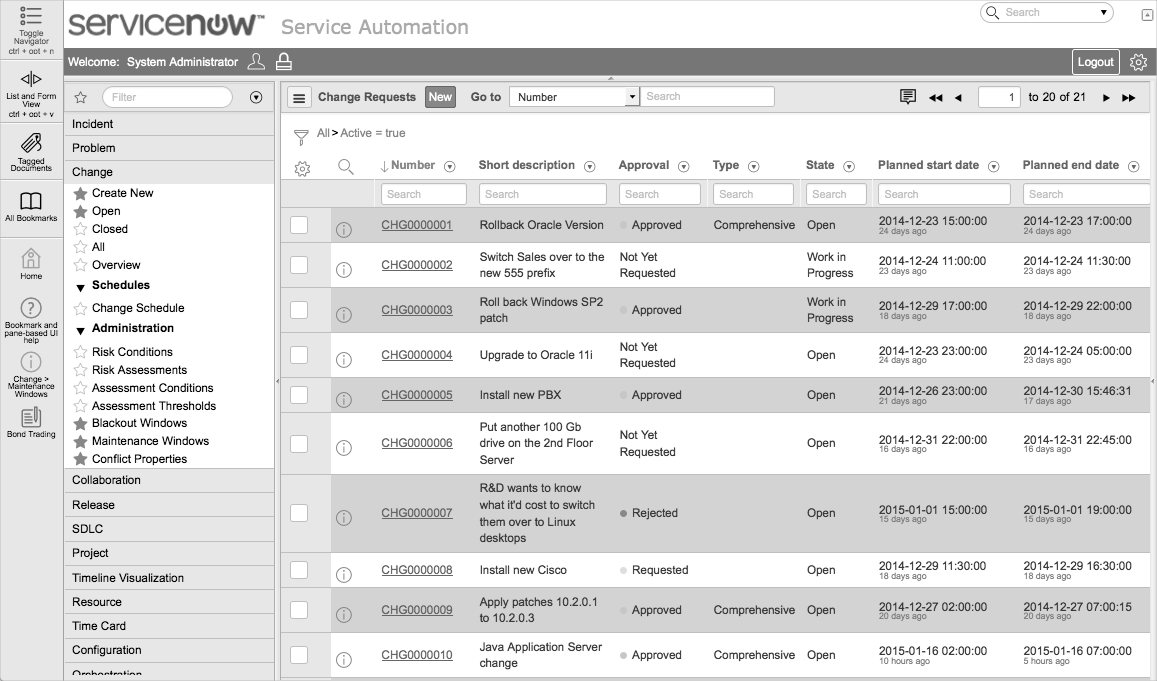
\includegraphics [scale=0.3] {svnow}
  \caption{Service NOW} 
  \label{img:svnow}  
\end{figure}

\textbf{IBMWatson}~--- это вопросно-ответная система, которая поддерживает понимание и формализацию запросов и поиск решений. Система не поддерживает автоматическое разрешение проблемы на основе формализации запроса. Система широко используется в медицине для постановки диагнозов болезней \cite{IBM1, IBM2, IBM3, IBM4} и реализует базовые принципы искусственного интеллекта \cite{IBM5, IBM6}. Ее разработка велась под суперкомпьютер IBM Deep Blue \cite{IBM7} группой под руководством профессора А. Гоэля. На рисунке \ref{img:Watson-Analytics} представлен общий вид этой системы. \par


\begin{figure} [h] 
  \center
  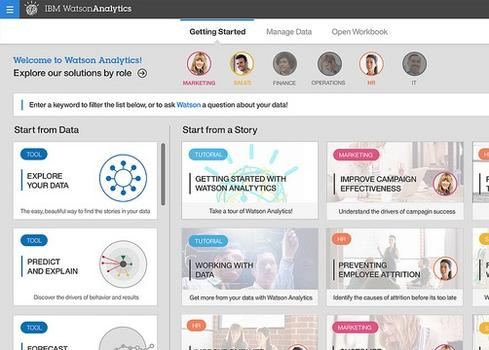
\includegraphics [scale=1.0] {Watson-Analytics}
  \caption{Пример работы системы Watson} 
  \label{img:Watson-Analytics}  
\end{figure}

Кроме того, известны следующие дополнительные способы и системы автоматизации разрешения проблемы пользователя:
\begin{itemize}
	\item Обработка инцидентов посредством регулярных выражений. В таком решении нет гибкости, так как обработка идет путем поиска ключевых слов вне контекста. Метод регулярных выражений частично используется для обработки естественного языка, поиска  \cite{REG1}, диагностики активных систем \cite{REG2}, анализа поведения функций \cite{REG4}, обработки данных в системе eDiscovery \cite{REG5}, в разработке способов программирования \cite{REG3};
	\item Обработка инцидентов при помощи скриптов~--- автоматизируются лишь рутинные операции.
\end{itemize} \par
На данный момент ни одна из описанных систем в полной мере автоматически не разрешает запросы пользователей: не фиксирует их, не проводит анализ, не ищет решение, не применяет решение и не дает обратную связь пользователю. Каждая система в той или иной мере реализует те или иные функции, но системы, которая реализует их все, нет. 

\section{Основные требования к интеллектуальным системам регистрации и анализа проблемных ситуаций в ИТ-области} \label{sect3_2}
Для того чтобы создать модель системы, необходимо определить требования к ней или критерии, соответствие которым будет служить одним из доказательств состоятельности системы наряду с экспериментальными результатами. \par

Перечисленные ниже требования сформированы, исходя из возможностей специалистов службы поддержки, а также анализа проблем, которыми они занимаются. Большинство инцидентов – тривиальные и типичные, но все они разные. Для человека проблемы ”Please install Firefox” и ”Please install Chrome” идентичны, но с точки зрения формализации это не так~--- общее в них можно найти, взглянув на обобщение различающейся части: Firefox и Chrome являются пакетами программного обеспечения. \par 
Чтобы понять, каким требованиям должны соответствовать интеллектуальная система регистрации и анализа проблемных ситуаций в ИТ-области, нужно понять, что делает специалист службы поддержки. Специалист регистрирует проблему, понимает, ищет решение, проводя логические рассуждения и фиксируя в памяти удачное решение, и решает проблему. Итак, для того чтобы обеспечить полностью автоматическое разрешение инцидентов, интеллектуальная система регистрации и анализа проблемных ситуаций в ИТ-области должна соответствовать следующим критериям: осуществлять мониторинг ИТ-инфраструктуры пользователя; регистрировать инциденты; создавать цепи обработки (Workflow) инцидента; понимать и формализовать запросы пользователя на естественном языке; искать решение и применять найденное решение; обучаться алгоритму разрешения инцидента; уметь проводить логические рассуждения (обобщение, специализация, синонимичный поиск). \par
Из этого списка требований к системе важно выделить формализацию запросов на естественном языке. Ниже приведены результаты анализа разработок в области формализации запросов на естественном языке. 

\clearpage

\section{Сравнительный анализ методов и комплексов обработки текстов на естественном языке}


\subsection{Обработка эталонных текстов} \label{sect2_1}
В данном разделе проведен обзор обработчиков естественного языка. За основу были взяты инциденты, выгруженные из систем поддержки ИТ-инфраструктуры \icl. В силу специфики предметной области (информационные технологии) основным языком был выбран английский язык. Был сформирован список из типичных эталонных фраз, на которых тестировались обработчики естественного языка. Фразы были выявлены путем анализа существующих отчетов об инцидентах. Примерами инцидентов являются следующие запросы.\par
\textbf{Инцидент 1}.
\textit{
User had received wrong application. User has ordered Wordfinder Business Economical for her service tag 7Q4TC3J, there is completed order in LOT with number ITCOORD-18125. However she received wrong version, she received Wordfinder Tehcnical instead of Business Economical. Please assist (Пользователю было установлено неверное приложение. Пользователь заказал приложение "Wordfinder Business Economical"\  для ее запроса номер 7Q4TC3J. По нашим данным запрос выполнен, номер результата ITCOORD-18125. Однако, он получил неверную версию~--- он получил приложение "Wordfinder Tehcnical"\  вместо "Wordfinder Business Economical". Пожалуйста, помогите).\footnote{Здесь и далее в переводе оригинальные ошибки сохранены, дабы продемонстрировать сложность формализации запросов на естественном языке.}
}\par
\textbf{Инцидент 2}.
\textit{
Laptop~--- user has almost full C:\ but when he looks in the properties of the files and folders on C:\ they are only 40GB and he has a 55GB drive (Ноутбук~--- диск C:\ пользователя переполнен, но он посмотрел свойства C:\ и увидел, что имеется только 40GB, хотя пользотель установил накопитель на 55Gb).
}\par
\textbf{Инцидент 3}.
\textit{
User cannot find Produkt Manageron start menu. Please reinstall (Пользователь не может найти Produkt Manageron в меню "Пуск". Пожалуйста, переустановите). 
}\par
\textbf{Инцидент 4}.
\textit{
User needs to have pdf 995 re-installed please (Пользователю нужно переустановить "pdf 995").
}\par

При анализе были использованы следующие обработчики естественного языка: Open NLP \cite{OpenNLP}, Relex\cite{OpenCogRelex}, StanfordParser \cite{StanfordParser}. Результат их работы оценивался при помощи метрик, представленных в таблице \ref{Metrics}, а полученные результаты приведены на рисунке \ref{img:ParserComp}. 

\begin{longtable}{|p{2cm}|p{6cm}|p{8cm}|}
 \caption[Таблица метрик]{Таблица метрик}\label{Metrics} \\ 
 \hline
 
 \multicolumn{1}{|c|}{\textbf{Метрика}} & \multicolumn{1}{c|}{\textbf{Описание}} & \multicolumn{1}{c|}{\textbf{Формула}} \\ \hline 
\endfirsthead
\multicolumn{2}{c}%
{{\bfseries \tablename\ \thetable{} -- продолжение}} \\
\hline\multicolumn{1}{|c|}{\textbf{Метрика}} & \multicolumn{1}{c|}{\textbf{Описание}} & \multicolumn{1}{c|}{\textbf{Формула}}  \\ \hline 
\endhead
\endfoot

\hline \hline
\endlastfoot
  \hline

Precision	& Точность & 
$$ 
P=\frac{tp}{tp+fp},
$$ где P~--- precision, tp~---  успешно обработанные слова, fp~--- ложно успешные \\
 \hline
Recall	& Чувствительность & 
$$ 
R=\frac{tp}{tp+fn},
$$ где R~--- recall, tp~--- успешно обработанные слова, fn~--- ложно неуспешные \\
 \hline
F	& F~--- measure (результативность) & 
$$ 
F=\frac{P*R}{P+R},
$$ где P~--- precision, R~--- recall.   \\
 
\end{longtable}

\begin{figure} [h] 
  \center
  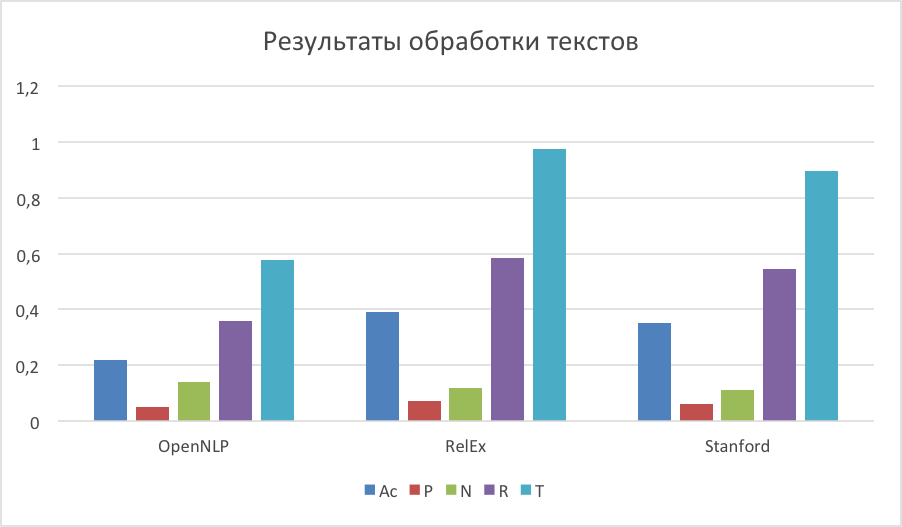
\includegraphics [scale=0.8] {ParserCompare}
  \caption{Результаты обработки текстов} 
  \label{img:ParserComp}  
\end{figure}

Из диаграммы видно, что наилучшие результаты показывает обработчик Relex\cite{OpenCogRelex}. После анализа необработанных инцидентов у всех обработчиков были выявлены проблемы двух типов:
\begin{enumerate}
	\item невозможность корректировки простых грамматических ошибок, связанных с пропущенными пробелами или неверным форматированием (ошибки первого типа);
	\item неверная интерпретация слов в предложении, например, слово please интерпретировалось как глагол, хотя является по смыслу «формой вежливости» (ошибки второго типа).
\end{enumerate}	\par

Несмотря на хорошие результаты~--- 63\% успешно разобранных предложений, ошибки первого и второго типов серьезно ухудшают результат. Эффективность разбора предложений в 63\% случаев недостаточна для успешной работы системы. Чтобы улучшить показатель, был разработан комплекс мер для устранения ошибок первого и второго типов.
	
 
\subsection{Исправление ошибок первого и второго типов} \label{sect2_2}
Чтобы разрешить проблемы, связанные с ошибками первого и второго типов, была проведена предварительная обработка текста, состоящая из 2-х фаз: комплексная корректировка для ошибок первого типа; обработка при помощи внутренней базы знаний для ошибок второго типа. 
Чтобы избавиться от орфографических, грамматических и синтаксических ошибок, был сконструирован составной корректировщик, который имеет модульную структуру и осуществляет корректировку последовательно. В результате были сконструированы модули корректировки: Google API~--- модуль подключения к открытым системам Google для использования их алгоритмов корректировки; After the Deadline~--- модуль, использующий открытый программный продукт After the Deadline для исправления текстов. 

Таким способом удалось исправить большинство ошибок, связанных с синтаксисом, грамматикой и орфографией. Также удалось исправить ошибки неверного написания: наличия лишних пробелов, пропуска запятых и точек. Но по-прежнему осталась проблема обработки неверной интерпретации слов в тексте. \par

Для корректировки ошибок второго типа был сконструирован модуль для обработчика естественного языка Relex, который разбивал стандартный процесс обработки на «предобработку» и «обработку». Стадия «обработки» включает в себя такой же алгоритм работы, как был до этого в модуле, а стадия «предобработки» проверяет входные данные (слово или предложение) на предмет его вхождения во внутреннюю базу знаний, и если таковое имеется, то приложение передает соответствующие корректировки обратно в модуль. Например, Relex во фразе "please install firefox"\ считает, что "please"\ --- это глагол, поэтому базе знаний нашей системы отмечено, что "please"\ --- это форма вежливости, тем самым Relex больше не интерпретирует "please"\ как глагол.


\subsection{Сравнение средств обработки русского и английского языков} \label{sect2_3}
Средства обработки естественного языка принято относить к большому классу средств NLP – Natural Language Processing \cite{NLP}. Для английского языка существует множество открытых средств обработки естественного языка, для русского языка найти их гораздо сложнее. Рассмотрим архитектуру средств обработки естественного языка на примере популярного комплекса обработки естественного языка~--- OpenCog Relex. \par
OpenCog Relex использует результаты работы открытого компонента для лексического анализа под названием Link Grammar \cite{linkgrammar}. Он поддерживает множество языков: английский, русский, турецкий, немецкий \etc\  В качестве формата вывода Relex использует синтаксис Link Grammar и преобразует его в формат связей, как показано в примере 1. Разбор примера приводится далее. 

\textbf{Пример 1}. User is unable to start KDP web, please reinstall Java.\\
\textbf{Результат} 
\begin{lstlisting}
_obj(start, KBP)
pos(start, verb)
inflection-TAG(start, .v)
tense(start, present)
pos([web], WORD)
noun_number(KBP, singular)
definite-FLAG(KBP, T)
pos(KBP, noun)
_advmod(reinstall, please)
pos(reinstall, verb)
inflection-TAG(reinstall, .v)
tense(reinstall, present)
pos(please, adv)
inflection-TAG(please, .e)
noun_number(Java, singular)
definite-FLAG(Java, T)
pos(Java, noun)
pos(., punctuation)
_obj(,, Java)
pos(,, verb)
tense(,, infinitive)
HYP(,, T)
_to-do(unable, ,)
pos(unable, adj)
inflection-TAG(unable, .a)
tense(unable, present)
pos(to, prep)
inflection-TAG(to, .r)
pos(be, verb)
inflection-TAG(be, .v)
_predadj(User, unable)
noun_number(User, singular)
definite-FLAG(User, T)
pos(User, noun)
\end{lstlisting}




Далее возьмем разбор слова start. В результате мы получим несколько отношений:
\begin{itemize}
	\item pos(start, verb)~--- start глагол;
	\item tense(start, present)~--- время настоящее;
	\item inflection-TAG(start, .v)~--- метод обозначения на схеме (индекс).
\end{itemize} \par
Остальные обработчики пока не поддерживают русский язык. Существуют открытые проекты, но они еще недостаточно развиты. Таковым является, например, русский словарь для LinkGrammar \footnote{\url{http://www.abisource.com/projects/link-grammar/russian/}}, но он не доступен для скачивания. 




\section{Выводы по главе 1}
В данной главе рассмотрены существующие на данный момент интеллектуальные системы регистрации и анализа проблемных ситуаций, возникающих в процессе функционирования ИТ-инфраструктуры предприятия.
 В таблице \ref{Comparsion} приведены сводные данные по системам. По ним можно сказать, что ни одна из рассмотренных систем полностью не реализует все необходимые функции для интеллектуальной системы разрешения проблемных ситуаций в ИТ-инфраструктуре предприятия. В главе 1 также выработаны критерии сравнения обработчиков естественного языка и выполнен анализ средств обработки естественного языка. По полученным показателям эффективности было решено использовать OpenCog Relex.

\begin{longtable}{|p{6cm}|p{0.5cm}|p{0.5cm}|p{0.5cm}|}
 \caption[Сравнительный анализ функциональности существующих решений]{Сравнительный анализ функциональности существующих решений}\label{Comparsion} \\ 
 \hline
 
 \multicolumn{1}{|c|}{\textbf{Сравнительный пункт}} & \multicolumn{1}{c|}{\textbf{HP Open View}} & \multicolumn{1}{c|}{\textbf{ServiceNOW}} & \multicolumn{1}{c|}{\textbf{IBM Watson}} \\ \hline 
\endfirsthead
\multicolumn{2}{c}%
{{\bfseries \tablename\ \thetable{} -- продолжение}} \\
\hline \multicolumn{1}{|c|}{\textbf{Сравнительный пункт}} & \multicolumn{1}{c|}{\textbf{HP Open View}} & \multicolumn{1}{c|}{\textbf{ServiceNOW}} & \multicolumn{1}{c|}{\textbf{IBM Watson}}  \\ \hline 
\endhead

\hline \multicolumn{2}{|r|}{{Продолжение следует}} \\ \hline
\endfoot

\hline \hline
\endlastfoot
\hline
   Мониторинг & Да & Да & Да \\
   \hline
   Регистрация инцидентов & Да & Да & Да\\
   \hline
   Управление системами & Да & Нет & Нет \\
   \hline 
   Создание цепи обработки (Workflow) инцидента & Да & Да & Нет \\
   \hline 
   Понимания и формализация запросов на естественном языке & Нет & Нет & Да \\
   \hline 
   Поиск решений & Нет & Нет & Да \\
   \hline 
   Применение решений & Нет & Нет & Нет \\
   \hline
   Обучение разрешению инцидента & Нет & Нет & Да \\
   \hline
   Умение проводить логические рассуждения: генерализацию, специализацию, синонимичный поиск & Нет & Нет & Нет \\
   \hline
   
\end{longtable}
\clearpage
